\section{Results}

\subsection{Validation of the controls}

When conducting \acrlong{de} analysis, the user has to ensure that controls are separated from the the tumours.
Homogeneity among the controls, similarity between the control and tumour counts distribution are also factors that can improve the results.
Despite that the controls should be separated from the tumours, it has been observed for different types of cancer in \acrshort{tcga} that the gene expression follows a similar distribution between the two conditions \cite*{Decamps2021}.

\begin{figure}
    \begin{center}
        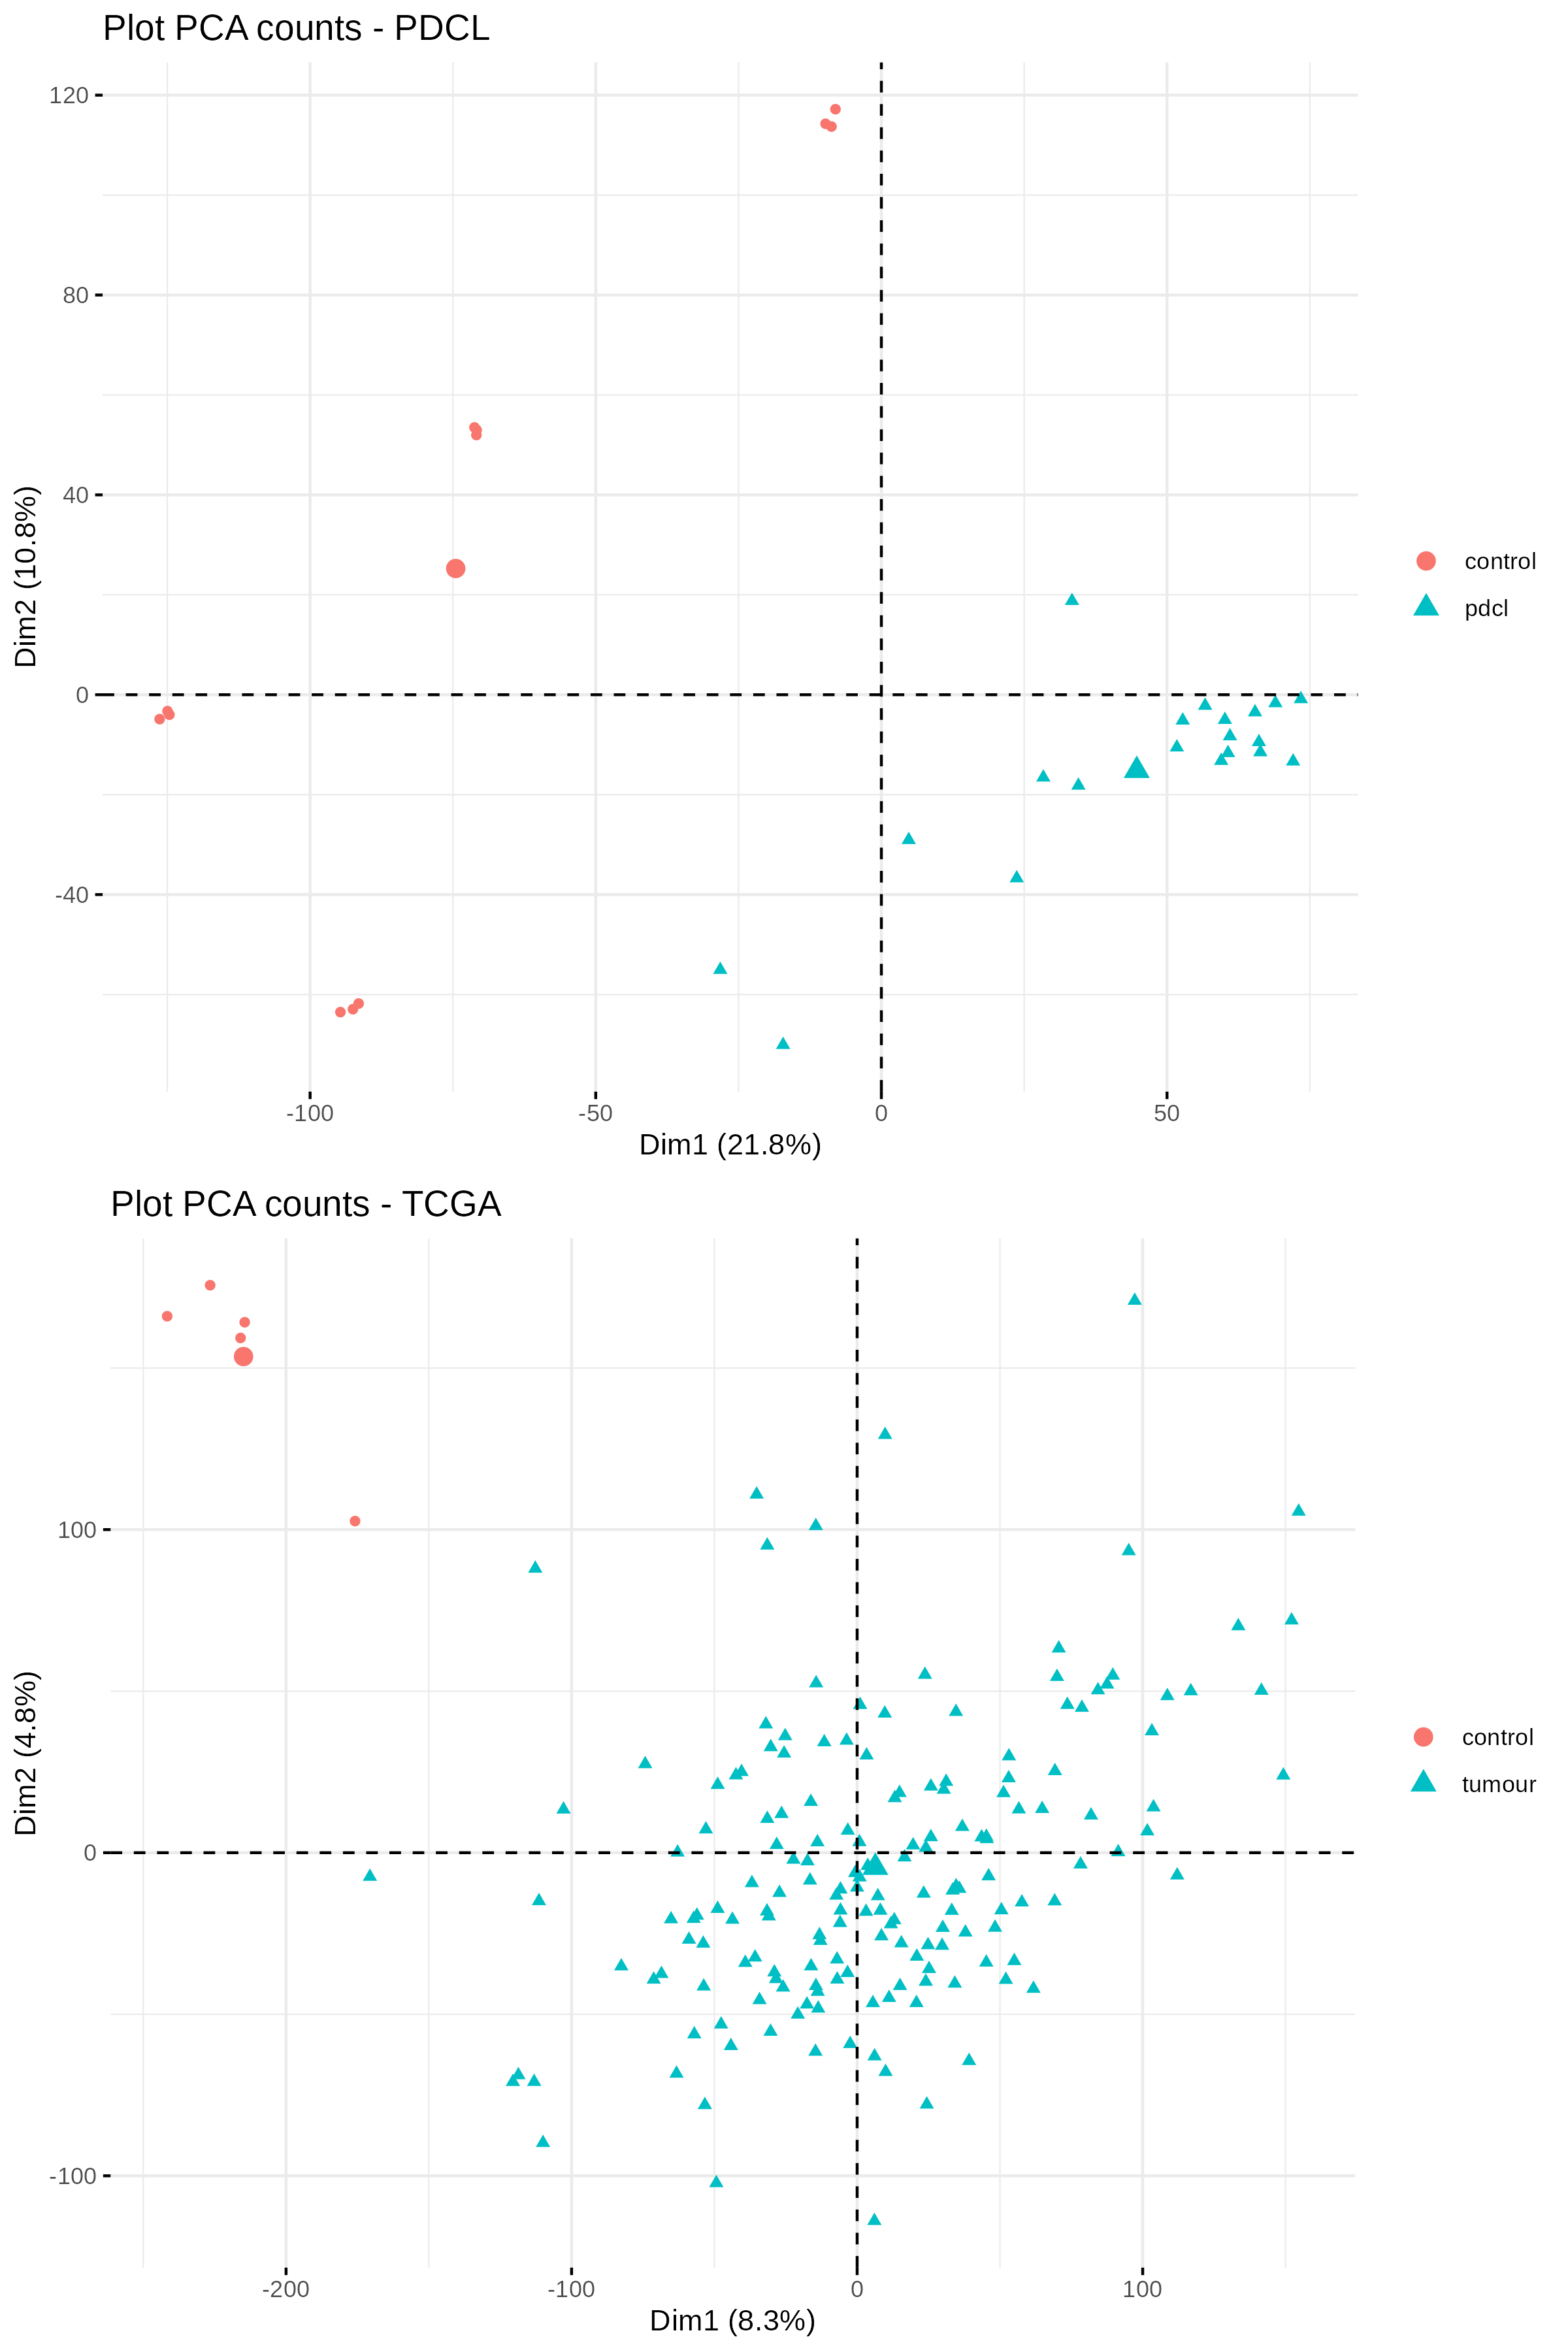
\includegraphics[height=0.8\textheight]{img/pca_plot}
        \caption{
            Plot of the \acrshort{pca} on the counts of control and glioblastoma samples of the \acrshort{pdcl} and \acrshort{tcga} datasets.
            Counts were normalized using the pseudo-log method of the DESeq2 package ( $log_2(count+1)$ ).
        }
        \label{fig:pca-plot}
    \end{center}
\end{figure}

Figure \ref*{fig:pca-plot} shows the results of a \acrfull{pca} performed on the counts normalized using the pseudo-log method from the DESeq2 package ( $log_2(count+1)$ ).
It can be seen that the controls are separated from the tumours  in both the \acrshort{pdcl} and the \acrshort{tcga} datasets by the first two components of the \acrshort{pca}.
The first component explain more variances in the data in the \acrshort{pdcl} datasets with 21\% compared to 8\% with \acrshort{tcga}.
In the \acrshort{tcga} datasets, the tumours samples tend to spread more accross the second component than the controls which seems to pack together while in the \acrshort{pdcl} dataset, controls are more scattered. 

\begin{figure}
    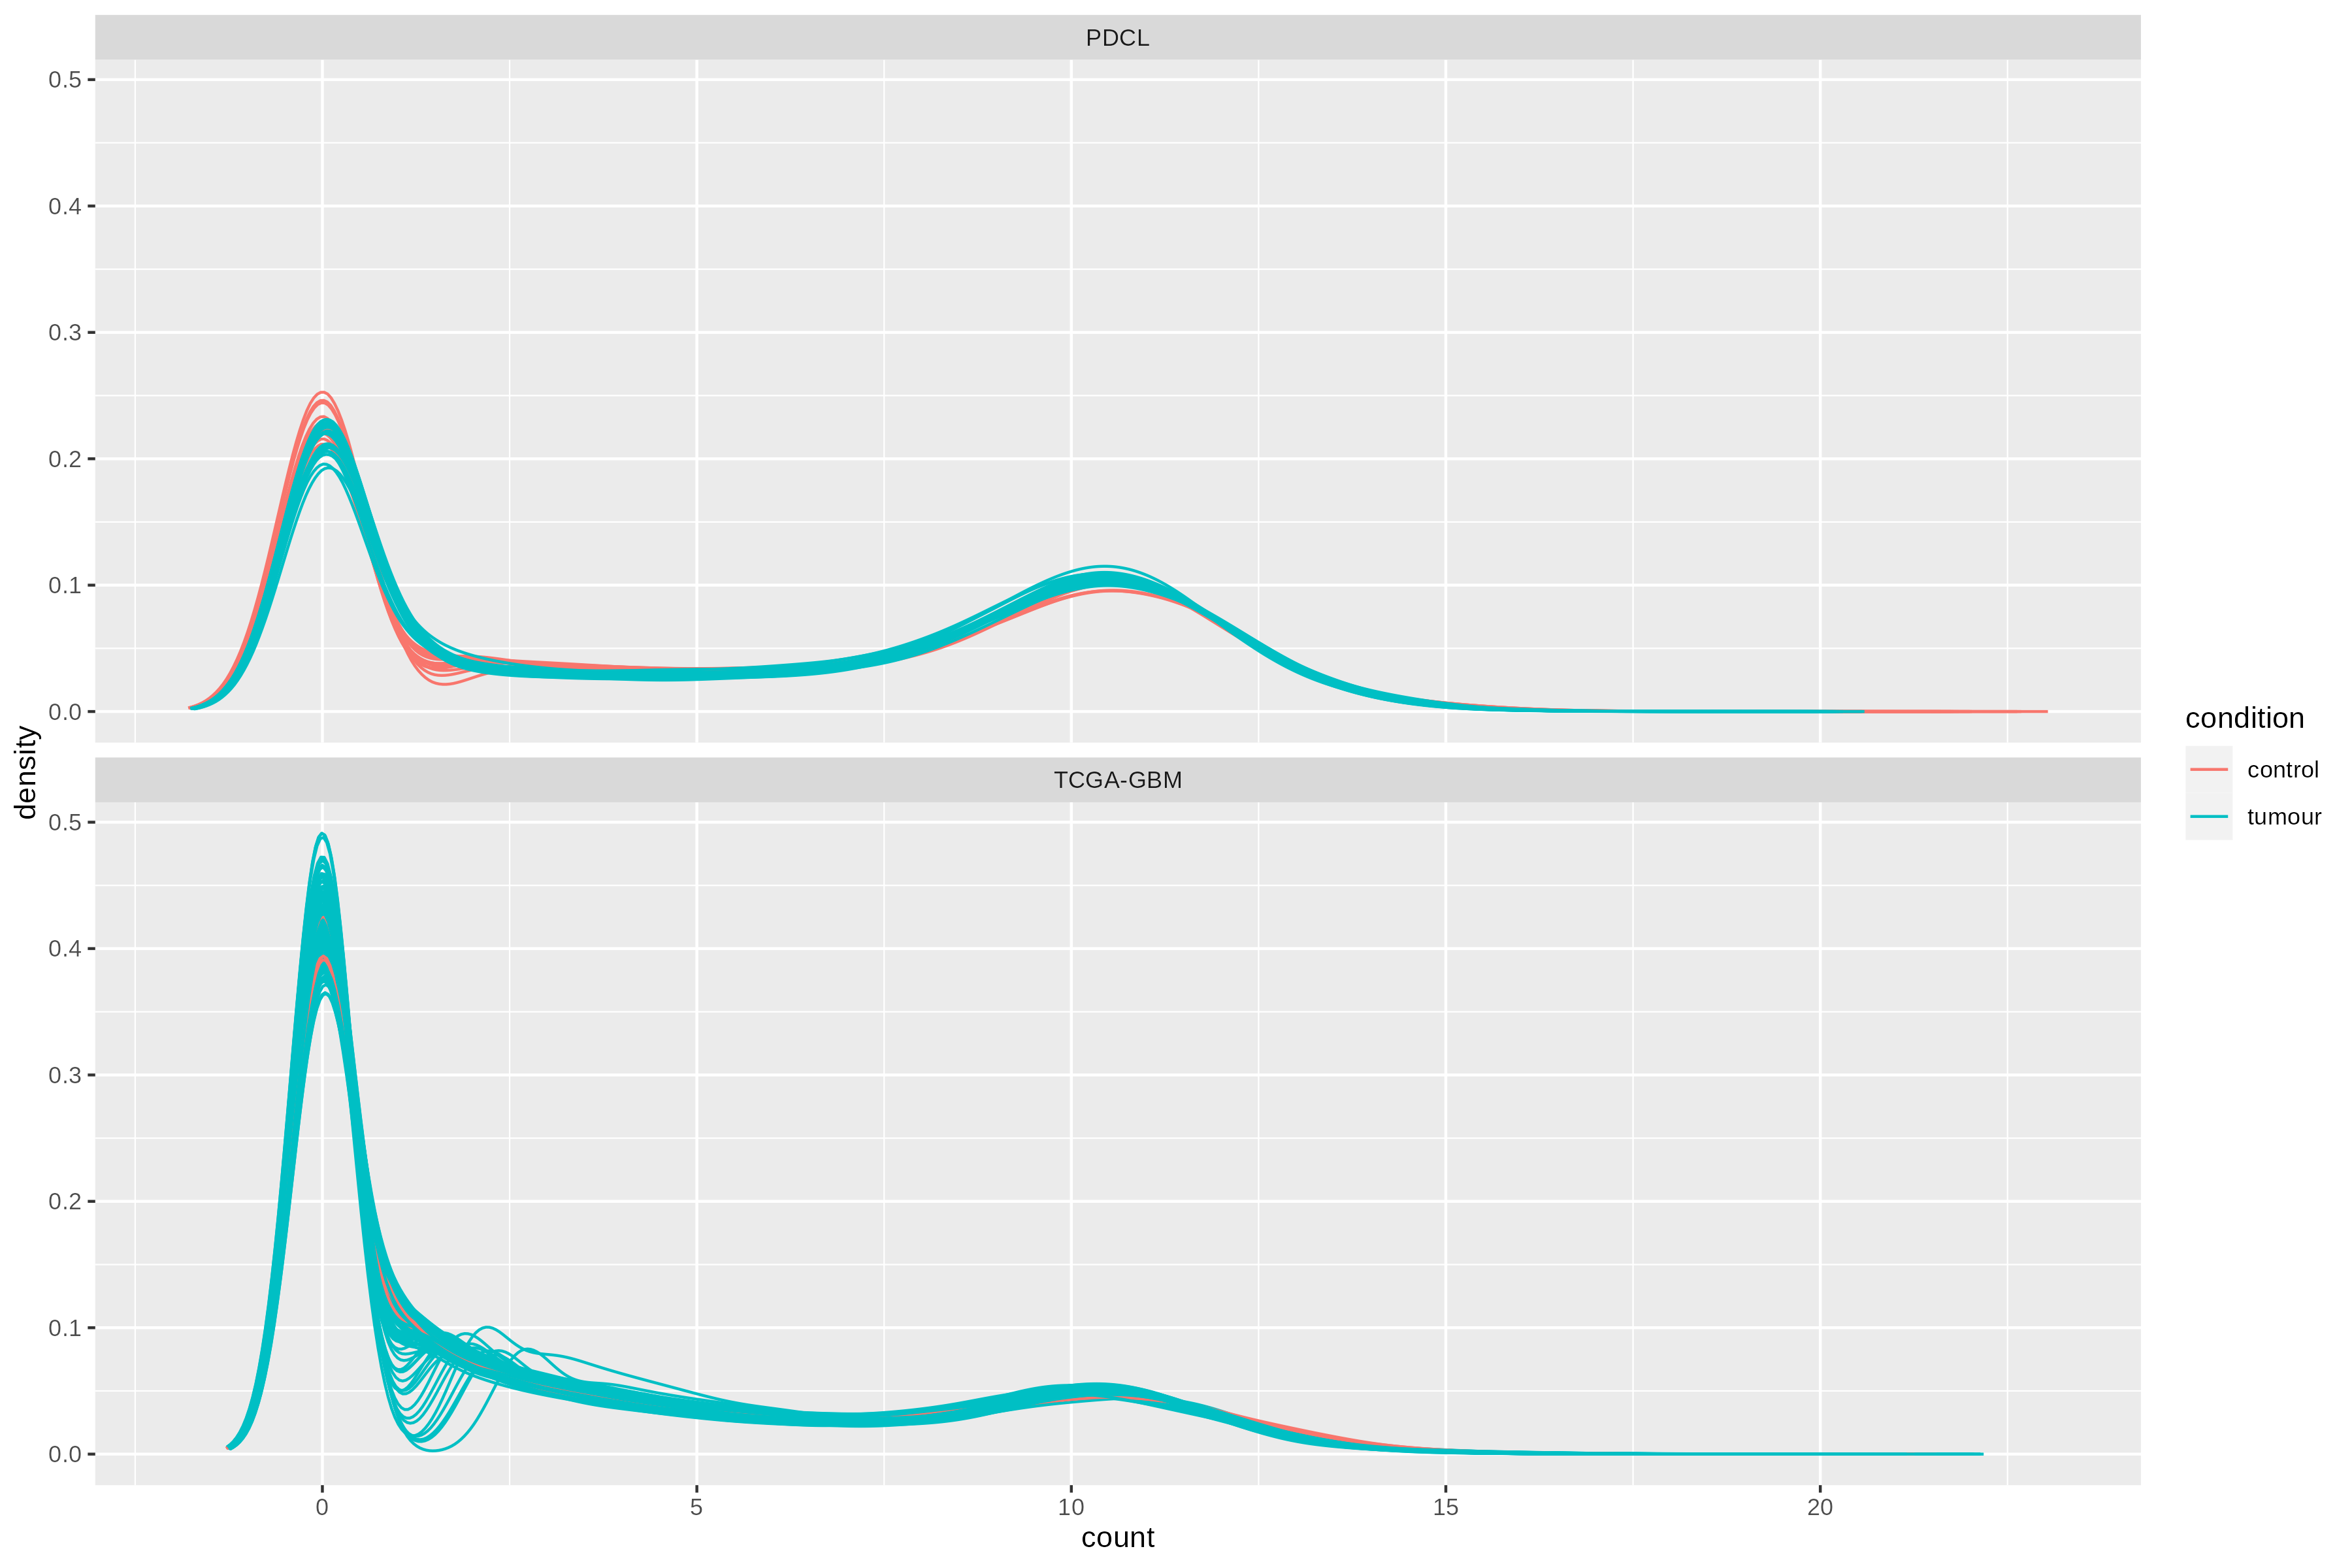
\includegraphics[width=\textwidth]{img/density_plot}
    \caption{
        Plot of the density of the counts in control and glioblastoma samples of the \acrshort{pdcl} and \acrshort{tcga} datasets.
        Counts were normalized using the pseudo-log method of the DESeq2 package ( $log_2(count+1)$ ).
        Each lines represent a different sample.
    }
    \label{fig:density-plot}
\end{figure}

Figure \ref*{fig:density-plot} shows the distribution of normalized gene counts in controls and tumours among both datasets.
Distribution of counts is similar among controls and tumours in both datasets with a similar intensity on the peak between controls and tumours with respect to the dataset.

Together, these data seems to indicate that the controls choosen are suitable to perform the \acrlong{de} analysis then pathway enrichment.

\subsection{Comparison of the deregulated pathways in the PDCL with the TCGA-GBM datasets}

\subsubsection{Pathways mainly involved in the Cell-Cycle, DNA replication and Repair are shared between the two datasets}

The \acrshort{kegg} database document the processes affected in the case of many diseases including glioma.
Zyla \textit{et al} used the \textit{Glioma} entry (path:hsa05214) as a target pathway to assess the sensitivity of different ranking metrics when studying microarray data from brain tissue \cite*{Zyla2017}.
They used the p-value associated with the enriched pathway to assess the sensitivity of each method.
To recall, the p-value indicates how significantly enriched a pathway is, the lower the better.
Therefore, for the target result \textit{glioma}, the p-value should be very low when studying RNA-Seq data from glioblastoma.
We here use the \acrshort{fdr}, an adjusted p-value to correct for multiple hypothesis testing, to determine the sensitivity of G:Profiler and \acrshort{gsea} in our analysis.
Here, \acrshort{fdr} value for this pathway in G:Profiler is 0.008898 for \acrshort{pdcl} and 0.05240 for \acrshort{tcga}, in \acrshort{gsea} it is 0.004487 for \acrshort{pdcl} and 0.8298 for \acrshort{tcga}.
Not only the \acrshort{fdr} value is lower for the \acrshort{tcga} dataset but the \acrshort{fdr} of \acrshort{gsea} for \acrshort{pdcl} does not pass the threshold defined in this study.
Even if the \acrshort{fdr} value was below the threshold in G:Profiler for the \textit{Glioma} target result in \acrshort{pdcl}, because it was above the threshold for G:Profiler we do not consider this result enriched in the \acrshort{pdcl} dataset.
Controls for the \acrshort{pdcl} dataset are taken from another study \cite*{Lundin2018}, introducing experimental and biological variability independent from disease deregulation.
While controls in the \acrshort{tcga} dataset come from matching samples taken off the original tissue following the exact same protocol as the tumour samples to reduce such variability.
It might explain why \acrshort{gsea} failed to detect the \textit{Glioma} entry in the \acrshort{pdcl} dataset.

Like the \textit{Glioma} target result, we only consider a pathway to be enriched in a dataset if the \acrshort{fdr} value for this pathway is below the threshold in both G:Profiler and \acrshort{gsea}.
Thus, only the pathways that meet this criterion are presented and discussed in the results.
45 pathways are found deregulated in the \acrshort{pdcl} dataset and 304 in the \acrshort{tcga} dataset.
As can be seen in the figure \ref{fig:heatmap-fdr-global-tcga}, the two datasets shared 19 significantly deregulated pathways which are involved in the cell-cycle, DNA repair and replication, gene expression, extracellular matrix and diseases.
\begin{figure}
    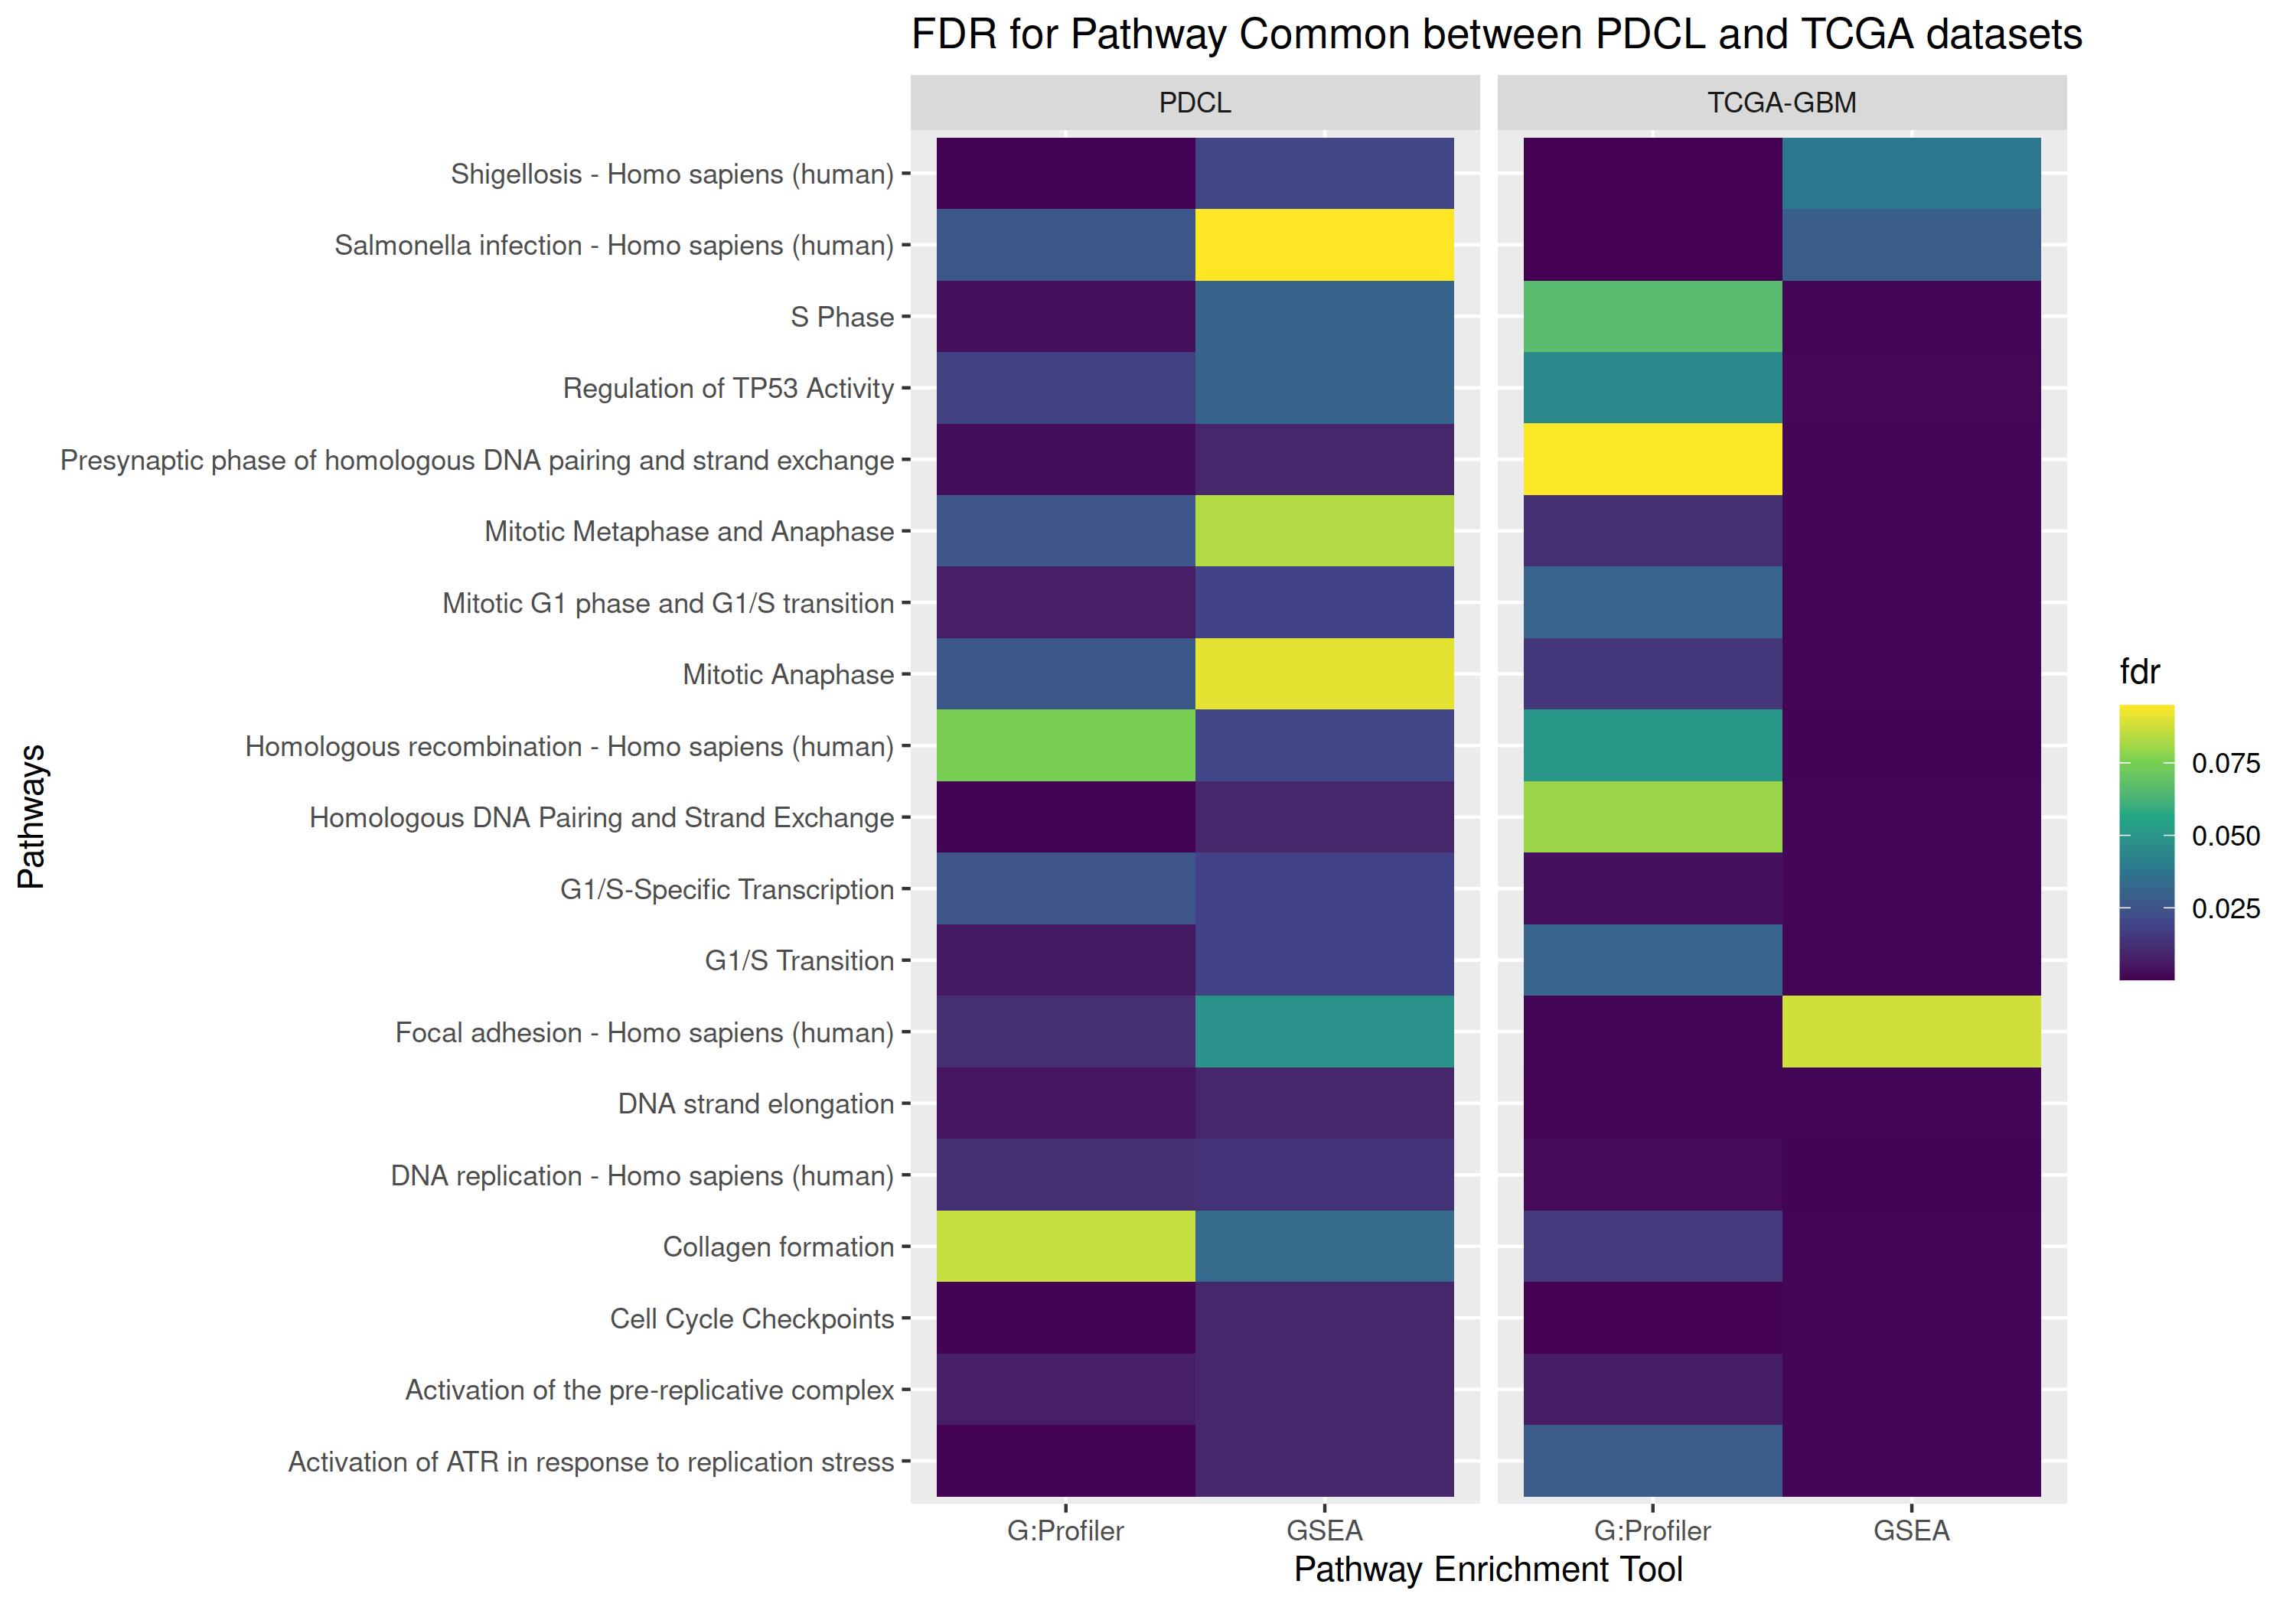
\includegraphics[width=\textwidth]{img/heatmap-fdr-global-tcga}
    \caption{
        \acrfull{fdr} of the pathways deregulated in both the \acrshort{pdcl} and the \acrshort{tcga} datasets.
        \acrshort{fdr} is lower than 0.1 since we only keep pathways below this value.
    }
    \label{fig:heatmap-fdr-global-tcga}
\end{figure}
The 2 pathways associated with disease (Shigellosis and Salmonella infection) belong to the \acrshort{kegg} database.
However, pathways involved in DNA replication and repair are significantly enriched for both \acrshort{kegg} and Reactome.
Interestingly, \textit{Regulation of TP53 activity} is found upregulated by \acrshort{gsea} for both datasets.
A study from \acrshort{tcga} on frequent mutations in glioblastoma has shown that p53 signalling is altered in 87\% of the samples and p53 is inactivated by mutation in 35\% of the samples \cite*{McLendon2008}.
Thus, the regulation of p53 may be upregulated to make up for the lack of activity from the mutated p53.

As can be seen in the figure \ref*{fig:complete-piechart-categ-pdcl}, the most deregulated category in the \acrshort{tcga} dataset is the \textit{Organismal Systems} category which includes biological processes involved in the Immune system, Endocrine system, Circulatory system, Digestive system, Sensory system, etc.
In the \acrshort{pdcl} dataset, \textit{Cell Cycle} is the most deregulated category in both the global and the personalized analysis (the analysis where each \acrshort{pdcl} samples are compared one by one to all the controls, lower panel in figure \ref*{fig:workflow-diagram-global}).
The \textit{Signal Transduction}, \textit{Metabolism of RNA and proteins} and the \textit{Cell-Cycle} categories are among the top 5 most deregulated categories in \acrshort{tcga}.
In comparison, less categories are affected in the global analysis for the \acrshort{pdcl} dataset, with \textit{DNA Processes} and \textit{Cell-Cycle} categories among the top 3 most deregulated categories.
In both \acrshort{tcga} and the global analysis of \acrshort{pdcl}, the \textit{Disease} category is the second most affected category.
\begin{figure}
    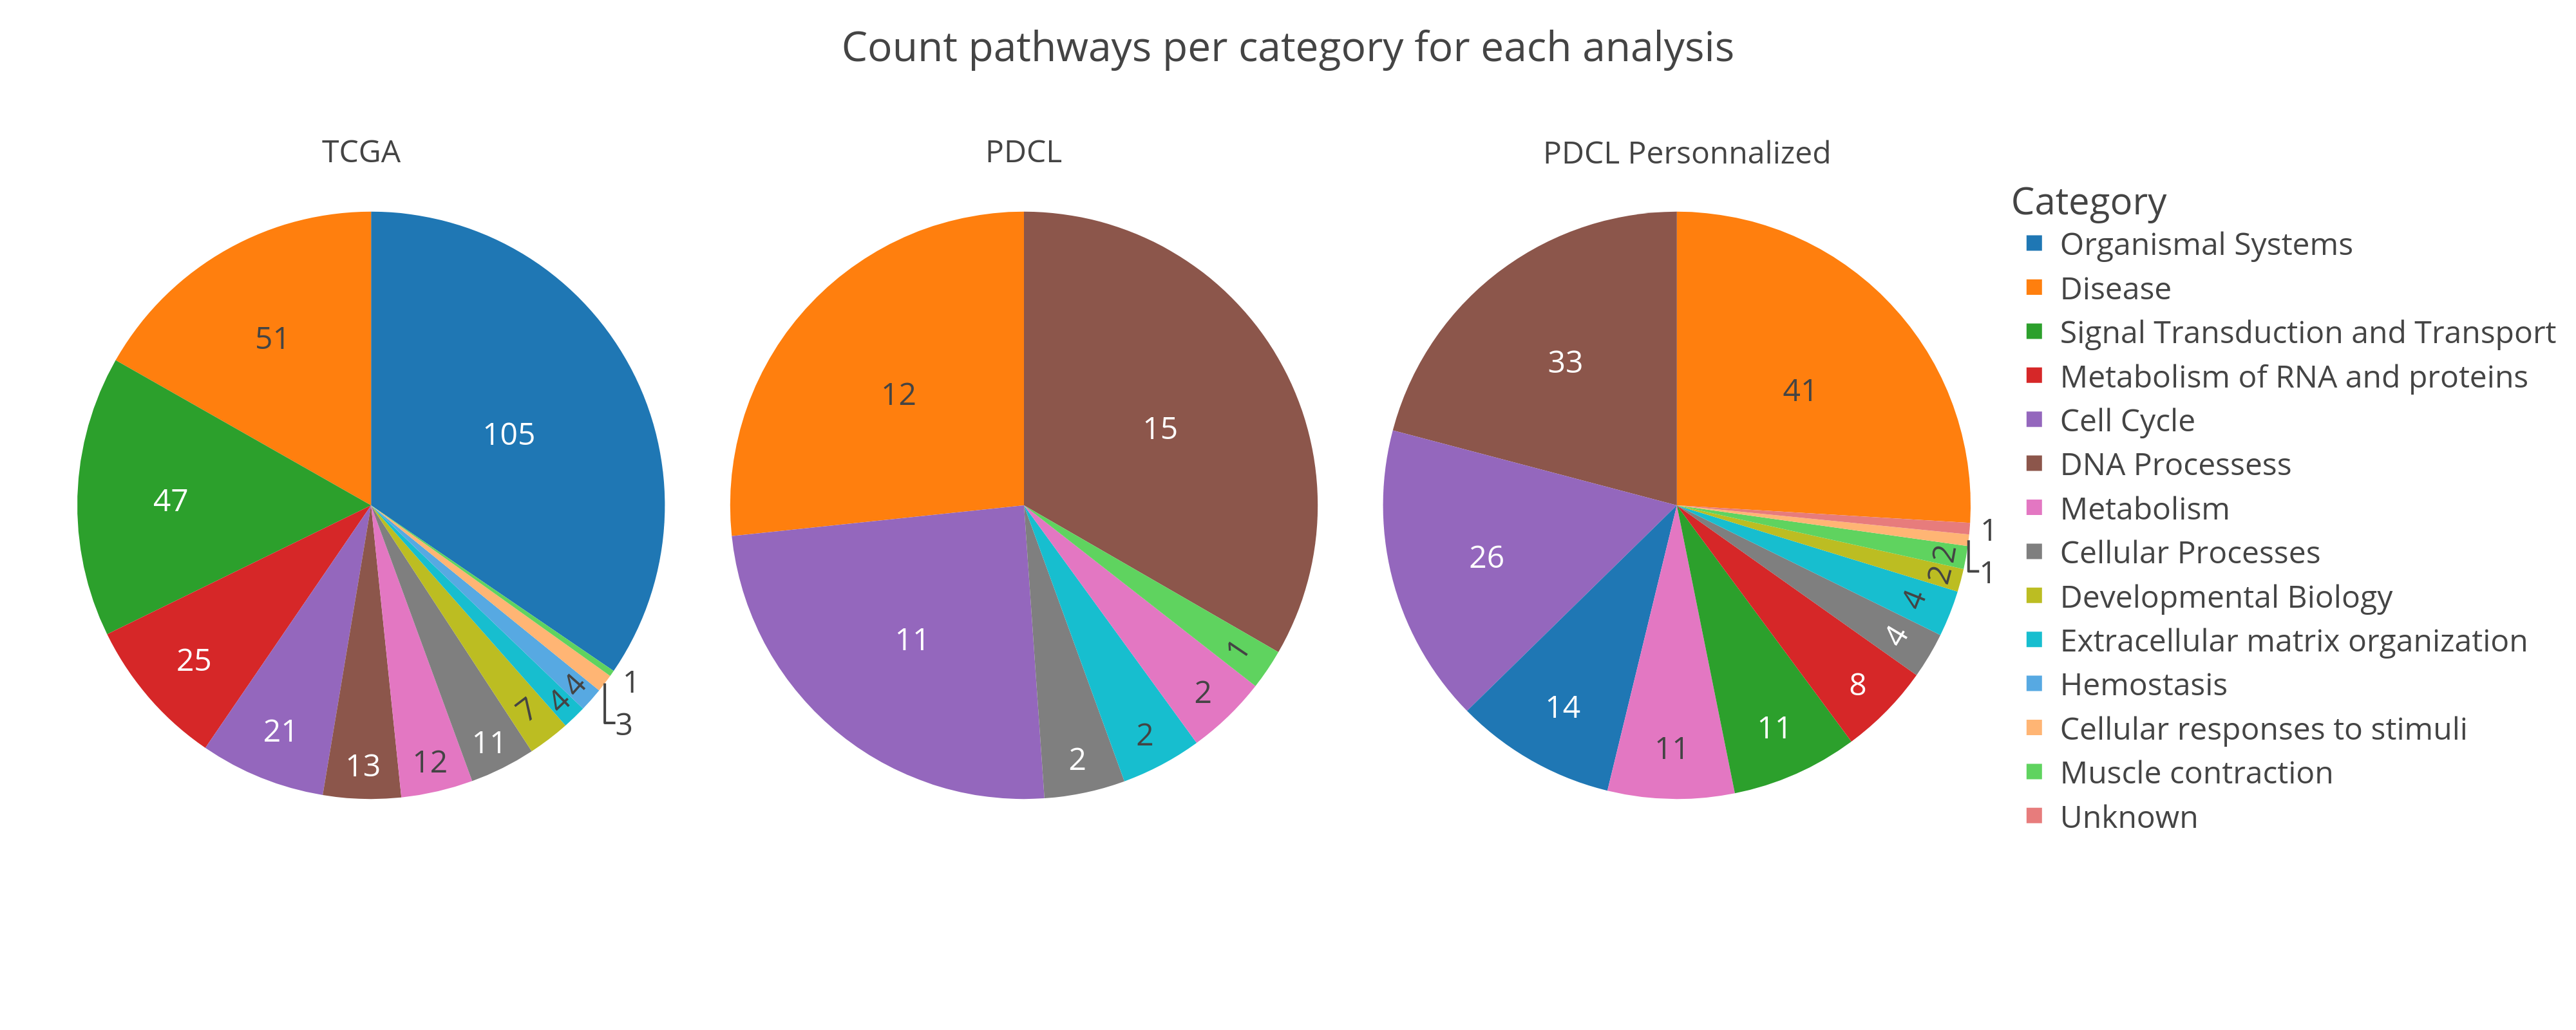
\includegraphics[width=\textwidth]{img/complete-piechart-categ-pdcl}
    \caption{
        Number of deregulated pathways per category and per analysis.
        The results are presented for the \acrshort{tcga} dataset, the global analysis and the personalized analysis of the \acrshort{pdcl} dataset.
        To recall, during the personalized analysis with compared each \acrshort{pdcl} samples against all the controls one by one (lower panel in figure \ref*{fig:workflow-diagram-global}).
        In the personalized analysis of the \acrshort{pdcl} dataset, only different results can contribute to the number of pathways for a category.
        Thus, a same pathway that is found deregulated in two different samples will only be counted once.
        The \textit{Organismal Systems} category includes pathways involved in the Immune system, Endocrine system, Circulatory system, Digestive system, Sensory system, etc.
        Among all analysis, the \textit{Disease} category is the first or the second most deregulated category.
        For \acrshort{tcga}, the top 5 most deregulated categories includes \textit{Organismal Systems}, \textit{Signal Transduction and Transport}, \textit{Metabolism of RNA and proteins} and \textit{Cell-Cycle}.
        While for the \acrshort{pdcl} dataset (global analysis), the most deregulated categories include \textit{Cell-Cycle} and \textit{DNA processeses}.
        The deregulated pathways in the personalized analysis of the \acrshort{pdcl} dataset mostly belong to the \textit{Cell-Cycle}, \textit{DNA processeses} and \textit{Organismal Systems}, \textit{Metabolism} and \textit{Signal Transduction and Transport}.
    }
    \label{fig:complete-piechart-categ-pdcl}
\end{figure}

\subsubsection{Cell-Cycle}

Two phases of the Cell Cyle are enriched in both datasets : the \textit{S phase} (R-HSA-69242) and the \textit{Mitotic Anaphase} (R-HSA-68882).
Interestingly, when in a first intention we kept pathways between 15 and 1,000 genes, \textit{Mitotic Anaphase}  was enriched only in \acrshort{tcga}.
It was enriched as well in the \acrshort{pdcl} dataset after we set up the boundary between 15 to 500 genes.
It highlights that the number of pathways present in the \acrshort{gmt} file has an impact on the significance of the results.

For both dataset, the \textit{Cell Cycle Checkpoints} pathway (R-HSA-69620) is affected.
Other pathways linked to the S phase of the cell-cycle are shared between datasets such as the \textit{DNA strand elongation} (R-HSA-69190) taking place in the S phase and the \textit{G1/S-Specific Transcription} (R-HSA-69205).

Among the pathways enriched only in the \acrshort{tcga} dataset, we found pathways that are children of pathways shared between both datasets.
For example, \textit{Amplification of signal from unattached kinetochores via a MAD2 inhibitory signal} (R-HSA-141444) is a children pathway of \textit{Cell Cycle Checkpoints} (R-HSA-69620), that is to say it is smaller pathway which takes place in its parent pathways.
Only G:Profiler's result for this pathway in the \acrshort{pdcl} dataset does not pass the threshold (\acrshort{fdr} is equal to 0.125).
We first hypothesized that the lower number of genes included in the \acrshort{pdcl} dataset (~20,000 genes compared to ~60,000 in \acrshort{tcga}) may be the cause.
Nonetheless, almost all the genes involved in this pathway are present in the \acrshort{pdcl} dataset.
A closer look at the number of genes that are deregulated and involved in this pathway shows 74 genes for \acrshort{tcga} compared to 48 for \acrshort{pdcl}, indicating that the number of deregulated genes is more likely to be at cause here.
This example may explain why other children processes taking place in a larger function are not detected in \acrshort{pdcl} compared to \acrshort{tcga} but may be affected.

\subsubsection{Metabolism}

Although pathways involved in metabolism are enriched in both datasets, none of them are shared between the two datasets.
The \acrshort{tcga} dataset is mostly enriched with pathways involved in the energetic metabolism such as \textit{Phospholipid metabolism} (R-HSA-1483257), \textit{Regulation of insuline secretion} (R-HSA-422356) and \textit{Selenoamino acid metabolism} (R-HSA-2408522).
The glycerophospholipid metabolism, part of phospholipid metabolism, is enriched in both Reactome and \acrshort{kegg} database.
The \acrshort{tcga} dataset is also enriched with pathways involved in the Metabolism of proteins or the Metabolism of RNA such as \textit{Peptide chain elongation} (R-HSA-156902), \textit{Translation initiation complex formation} (R-HSA-72649) and \textit{rRNA processing in the nucleus and cytosol} (R-HSA-8868773).

Compared to the \acrshort{tcga} dataset, there are no pathways involved in the Metabolism of proteins or the Metabolism of RNA enriched in the \acrshort{pdcl}.
The only pathway involved in metabolism found deregulated is the \textit{Cholesterol Biosynthesis} (R-HSA-191273) and the \textit{Steroid biosynthesis} (path:hsa00100), 2 pathways having a role in cholesterol metabolism.

\subsubsection{Extra-Cellular Matrix}

The \textit{Collagen formation} (R-HSA-1474290) and \textit{focal adhesion} (path:hsa04510) pathways are shared between the \acrshort{tcga} and \acrshort{pdcl} datasets.
They are related to the \acrlong{ecm} and the cell-matrix interactions as collagen is a protein composing the \acrshort{ecm} and the \textit{focal adhesion} is a process where the cell adheres to the matrix.
Only in the \acrshort{tcga} dataset, the \textit{Assembly of collagen fibrils and other multimeric structures} (R-HSA-2022090) and the \textit{Collagen biosynthesis and modifying enzymes} (R-HSA-1650814), two pathways included in the \textit{Collagen formation}, are found enriched.
The \textit{\acrshort{ecm}-receptor interaction} (path:hsa04512), \textit{Cell adhesion molecules} (path:hsa04514) and the \textit{Laminin interaction} (R-HSA-3000157) are pathways related to the adhesion of the cell to the \acrshort{ecm} only enriched in the \acrshort{tcga} datasets as well.
The \textit{Non-integrin membrane-ECM interactions} (R-HSA-3000171) is another pathway related to the \acrshort{ecm}-cell interactions yet only found enriched in the \acrshort{pdcl}.
The results seem to indicate that \acrshort{ecm} and cell adhesion carry a role in glioblastoma growth.
Since the \textit{Collagen formation} pathway is shared by the two datasets, it suggests that this process is important for glioblastoma growth.
However, \textit{Laminin interaction} and \textit{Non-integrin membrane-ECM interactions}, two pathways classified on the same level in the hierarchy of Reactome, tend to show different mechanisms by which the tumour cell can influence its adhesion to the \acrshort{ecm}.
Surprisingly, \textit{Focal adhesion} and \textit{Collagen formation} were both upregulated in \acrshort{tcga} but downregulated in \acrshort{pdcl}.
This may be due to the controls used in the \acrshort{pdcl} dataset.

\subsection{Analysis of the deregulated pathways at the individual level}

\subsubsection{Cell adhesion to the ECM is the most frequently deregulated pathway in PDCL samples}

Table \ref*{table:frequently-dereg-pathways-kegg} and \ref*{table:frequently-dereg-pathways-reactome} show the most frequently deregulated pathways in \acrshort{pdcl}.
The \textit{Focal adhesion} (path:hsa04510) is the most frequently deregulated \acrshort{kegg} pathway with 13 samples affected while \textit{Transmission across Chemical Synapses} (R-HSA-112315) is the most frequently deregulated Reactome pathway with 5 samples affected.
Results contain pathways linked to processes influencing the cell motility and its fixation on the matrix such as :\textit{Focal adhesion} (path:hsa04510), \textit{ECM-receptor interaction} (path:hsa04512), \textit{Cell adhesion molecules} (path:hsa04514), \textit{Collagen synthesis} (R-HSA-165814, R-HSA-8948216) and \textit{elastic fibre formation} (R-HSA-1566948).
Glioblastoma cells have the ability to migrate and invade surrounding tissue, sometimes migrating to other organs as well \cite*{Lah2020}, confirming the validity of these results.

In a similar way, \textit{Steroid biosynthesis} and \textit{Cholesterol biosynthesis} are found deregulated in 4 and 3 different samples, respectively.
As we will described more in the Discussion section, cholesterol metabolism has been documented in the litterature to be affected in the case of glioblastoma.

The \textit{Oxidative phosphorylation} (path:hsa00190), well-known for its role in the generation of \acrshort{atp}, is found deregulated in 4 samples.
This pathway has been widely studied due to its important role in the generation of \acrshort{atp} and its potential implication in the Warburg Effect, an increase of usage of glycolysis to produce \acrshort{atp} even though oxygen is available \cite*{Spinicci2022}.
It was first hypothesized that mitochondria were defective in tumour cells, yet it was later mitochondrial function was similar to normal cells \cite*{Cairns2011}.
The \textit{Hippo signaling pathway} (path:hsa04392, path:hsa04390) and \textit{Retrograde endocannnabinoid signaling} (path:hsa04723), two signaling pathway whose role in cancer have been documented in the litterature, are found deregulated in 6 and 5 different samples, respectively.
\todo{read the article about them before citing them as references}

\begin{table}
    \centering
    \resizebox*{\textwidth}{!}{
        \begin{tabular}{ |c|c|c|c|c| }
            \hline
            Database & Pathway ID & Description & Category & Number of PDCL \\
            \hline
            KEGG & path:hsa04510 & Focal adhesion & Cellular Processes & 13 \\
            KEGG & path:hsa04360 & Axon guidance & Organismal Systems & 10 \\
            KEGG & path:hsa04512 & ECM-receptor interaction & Environmental Information Processing & 5 \\
            KEGG & path:hsa04724 & Glutamatergic synapse & Organismal Systems & 5 \\
            KEGG & path:hsa04725 & Cholinergic synapse & Organismal Systems & 5 \\
            KEGG & path:hsa00100 & Steroid biosynthesis & Metabolism & 4 \\
            KEGG & path:hsa00190 & Oxidative phosphorylation & Metabolism & 4 \\
            KEGG & path:hsa04612 & Antigen processing and presentation & Organismal Systems & 4 \\
            KEGG & path:hsa04723 & Retrograde endocannabinoid signaling & Organismal Systems & 4 \\
            KEGG & path:hsa03008 & Ribosome biogenesis in eukaryotes & Genetic Information Processing & 3 \\
            KEGG & path:hsa04012 & ErbB signaling pathway & Environmental Information Processing & 3 \\
            KEGG & path:hsa04072 & Phospholipase D signaling pathway & Environmental Information Processing & 3 \\
            KEGG & path:hsa04392 & Hippo signaling pathway - multiple species & Environmental Information Processing & 3 \\
            KEGG & path:hsa04514 & Cell adhesion molecules & Environmental Information Processing & 3 \\
            KEGG & path:hsa04714 & Thermogenesis & Organismal Systems & 3 \\
            \hline
        \end{tabular}
    }
    \caption{
        Table of the frequently \acrshort{kegg} pathways deregulated in the \acrshort{pdcl}.
        \textit{Focal adhesion} is the most frequently deregulated pathway with 13 samples affected.
    }
    \label{table:frequently-dereg-pathways-kegg}
\end{table}

\begin{table}
    \centering
    \resizebox*{\textwidth}{!}{
        \begin{tabular}{|c|c|c|c|c|}
            \hline
            Database & Pathway ID & Description & Category & Number of PDCL \\
            \hline
            Reactome & R-HSA-112315 & Transmission across Chemical Synapses & Neuronal System & 5 \\
            Reactome & R-HSA-1650814 & Collagen biosynthesis and modifying enzymes & Extracellular matrix organization & 4 \\
            Reactome & R-HSA-5576891 & Cardiac conduction & Muscle contraction & 4 \\
            Reactome & R-HSA-8948216 & Collagen chain trimerization & Extracellular matrix organization & 4 \\
            Reactome & R-HSA-112314 & Neurotransmitter receptors and postsynaptic signal transmission & Neuronal System & 3 \\
            Reactome & R-HSA-191273 & Cholesterol biosynthesis & Metabolism & 3 \\
            Reactome & R-HSA-6790901 & rRNA modification in the nucleus and cytosol & Metabolism of RNA & 3 \\
            Reactome & R-HSA-6794362 & Protein-protein interactions at synapses & Neuronal System & 3 \\
            Reactome & R-HSA-109581 & Apoptosis & Programmed Cell Death & 2 \\
            Reactome & R-HSA-1296071 & Potassium Channels & Neuronal System & 2 \\
            Reactome & R-HSA-1566948 & Elastic fibre formation & Extracellular matrix organization & 2 \\
            Reactome & R-HSA-157579 & Telomere Maintenance & Cell Cycle & 2 \\
            Reactome & R-HSA-174417 & Telomere C-strand (Lagging Strand) Synthesis & Cell Cycle & 2 \\
            Reactome & R-HSA-187037 & Signaling by NTRK1 (TRKA) & Signal Transduction & 2 \\
            Reactome & R-HSA-204998 & Cell death signalling via NRAGE, NRIF and NADE & Signal Transduction & 2 \\
            \hline
        \end{tabular}
    }
    \caption{
        Table of the frequently Reactome pathways deregulated in the \acrshort{pdcl}.
        \textit{Transmission across Chemical Synapses} is the most frequently deregulated pathway with 5 samples affected.
        Collagen pathways are dysregulated in 4 different samples.
    }
    \label{table:frequently-dereg-pathways-reactome}
\end{table}

\begin{figure}
    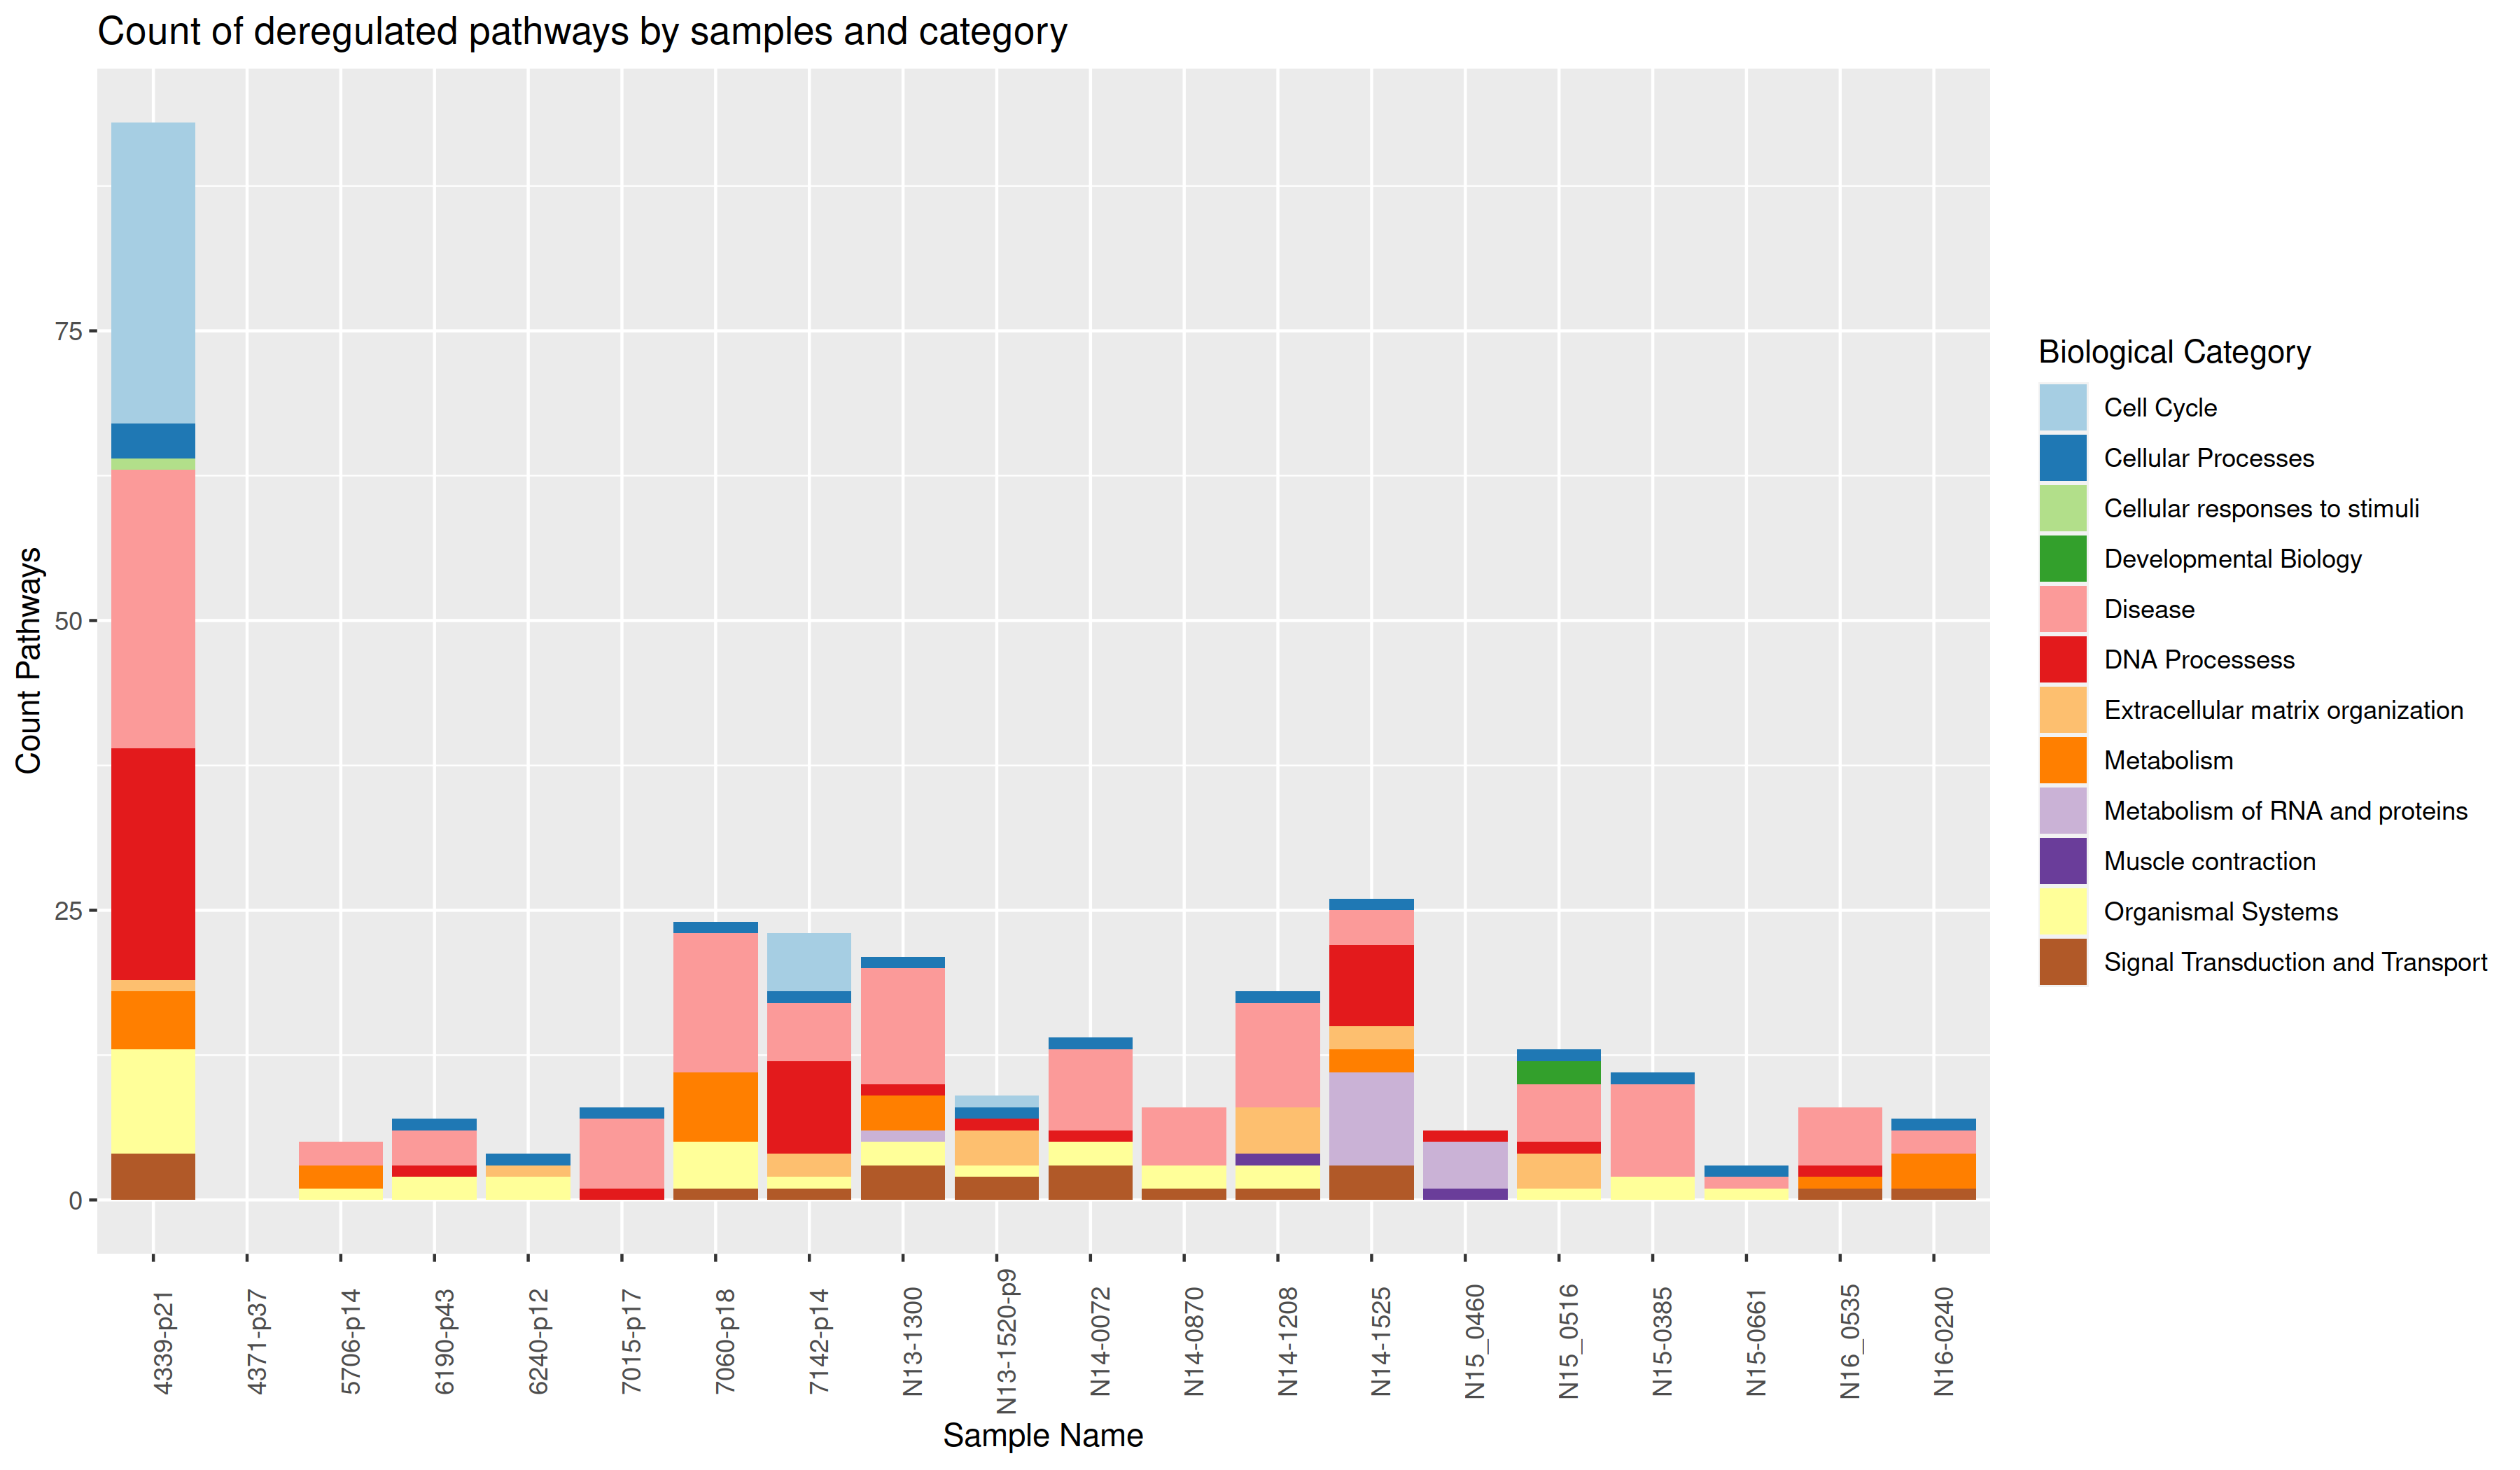
\includegraphics[width=\textwidth]{img/barplot-categ-pdcl}
    \caption{
        Number of deregulated pathways per category and per sample in the \acrshort{pdcl} dataset.
        The  \textit{Human Diseases} and \textit{Organismal Systems} categories are the most frequently deregulated \acrshort{kegg} categories.
        In Reactome, deregulated pathways are often associated with \textit{Neuronal System}, \textit{DNA Repair/Replication} and \textit{Signal Transduction}.
        \textit{4339-p21} is the the sample with the most deregulated pathways in both \acrshort{kegg} and reactome.
        Pathways in this sample are associated to the \textit{Cellular Processes} and \textit{Environmental/Genetic Information Processing} \acrshort{kegg}, or the \textit{Cell-Cycle} Reactome category.
    }
    \label{fig:barplot-categ-pdcl}
\end{figure}

As can be seen in figure \ref*{fig:barplot-categ-pdcl}, the sample \textit{4339-p21} is the most deregulated with around 40 pathways significantly enriched in both \acrshort{kegg} and Reactome.
Most of the pathway found deregulated with the \acrshort{kegg} database, across all the \acrshort{pdcl} samples, are associated to \textit{Human Diseases}.
\textit{Human Diseases} aside, the majority of deregulated pathways in the sample \textit{4339-p21} are associated to the \textit{Cellular Processes} and \textit{Environmental/Genetic Information Processing} \acrshort{kegg}, or the \textit{Cell-Cycle} Reactome category.